\documentclass{beamer}
\usetheme{Boadilla}

\makeatother
\setbeamertemplate{footline}
{
    \leavevmode%
    \hbox{%
    \begin{beamercolorbox}[wd=.4\paperwidth,ht=2.25ex,dp=1ex,center]{author in head/foot}%
        \usebeamerfont{author in head/foot}\insertshortauthor
    \end{beamercolorbox}%
    \begin{beamercolorbox}[wd=.55\paperwidth,ht=2.25ex,dp=1ex,center]{title in head/foot}%
        \usebeamerfont{title in head/foot}\insertshorttitle
    \end{beamercolorbox}%
    \begin{beamercolorbox}[wd=.05\paperwidth,ht=2.25ex,dp=1ex,center]{date in head/foot}%
        \insertframenumber{}
    \end{beamercolorbox}}%
    \vskip0pt%
}
\makeatletter
\setbeamertemplate{navigation symbols}{}

\usepackage{lmodern}
\usepackage{amssymb,amsmath}
\renewcommand{\familydefault}{\sfdefault}

\DeclareMathOperator*{\argmax}{argmax}

\usepackage{mathtools}
\usepackage{graphicx}
\usepackage{threeparttable}
\usepackage{booktabs}
\usepackage{siunitx}
\sisetup{parse-numbers=false}

% \setlength{\OuterFrameSep}{-2pt}
% \makeatletter
% \preto{\@verbatim}{\topsep=-10pt \partopsep=-10pt }
% \makeatother

\title[Week 1:\ Course Overview]{Week 1:\ Course Overview}
\author[Econ 590:\ Special Topics in Economics]{Econ 590:\ Special Topics in Economics}
\date{Anuar Assamidanov\\Cal State Fullerton}

\begin{document}

{\setbeamertemplate{footline}{} 
\begin{frame}[noframenumbering]
    \titlepage
\end{frame}
}

\section{Agenda}
\begin{frame}\frametitle{Agenda}
    Today's topics
    \begin{itemize}
    	\item \hyperlink{page.\getpagerefnumber{introductions}}{Introductions}
        \item \hyperlink{page.\getpagerefnumber{information}}{Course information}
        \item \hyperlink{page.\getpagerefnumber{materials}}{Course materials}
        \item \hyperlink{page.\getpagerefnumber{grades}}{Grades and assignments}
    \end{itemize}
\end{frame}


\section{Introductions}
\label{introductions}
\begin{frame}\frametitle{}
    \vfill
    \centering
    \begin{beamercolorbox}[center]{title}
        \Large Introductions
    \end{beamercolorbox}
    \vfill
\end{frame}

\begin{frame}\frametitle{My Info}
    Anuar Assamidanov
    \begin{itemize}
        \item Ph.D student, Applied Microeconomics
    \end{itemize}
    \vspace{2ex}
    Contact info
    \begin{itemize}
        \item Email: \href{aassamidanov@fullerton.edu}{\texttt{aassamidanov@fullerton.edu}}
        \item Office hours: Monday 5:30--6:30 pm, Tuesday 10-11 am (via Zoom)
    \end{itemize}
    \vspace{2ex}
    Best way to communicate with me
    \begin{itemize}
        \item ``Public'' question: Ask in class
        \item Short ``private'' question: Email with [Econ 590] in the subject
        \item Longer ``private'' question: Sign up for office hours
    \end{itemize}
\end{frame}

\begin{frame}\frametitle{About Me}
    \begin{itemize}
        \item I study labor economics, economics of crime, applied econometrics, and machine learning
        \item This is my second time teaching Machine Learning
        \begin{itemize}
            \item You can play a role in shaping the design of this course, for yourself and for future classes
        \end{itemize}
        \item Call me ``Anwar'' if you would like
        \item Pronouns: he/him/his
    \end{itemize}
\end{frame}

\begin{frame}\frametitle{About You}
    Introduce yourself
    \begin{itemize}
        \item Name
        \item Pronouns
        \item Department
        \item Research interests
        \item Favorite (or most familiar) statistical software? 
        \begin{itemize}
            \item Any experience with Python?
        \end{itemize}
        \item Anything else you want us to know?
    \end{itemize}
\end{frame}

\section{Course Information}
\label{information}
\begin{frame}\frametitle{}
    \vfill
    \centering
    \begin{beamercolorbox}[center]{title}
        \Large Course Information
    \end{beamercolorbox}
    \vfill
\end{frame}

\begin{frame}\frametitle{Course Website}
    \begin{center}
    	\href{https://github.com/assamidanov/econ_590}{\texttt{github.com/assamidanov/econ{\_}590}}
    \end{center}
    \vspace{3ex}
    I will use this GitHub repository to post lecture slides, Python code, problem sets, datasets, etc.
\end{frame}

\begin{frame}\frametitle{Course Description}
    You have already learnt
    \begin{itemize}
        \item Classical linear regression model
        \item ``Treatment effect'' estimation
    \end{itemize}
    (If you have not taken Elementary Statistics  {\&} Econometrics, please see me to determine if this course is appropriate for you) \\
    \vspace{3ex}
This introductory course gives an overview of different concepts, techniques, and algorithms in machine learning (ML) and their applications in an economic setting. We begin with classification, linear and non-linear regressions, bagging, boosting, and end with more recent neural networks and deep learning models. We will also touch on the recent methods at the intersection of ML and econometrics, designed for causal inference, optimal policy estimation, estimation of
counterfactual effects.
\end{frame}

\begin{frame}\frametitle{Course Goals}
    \begin{enumerate}
        \item Gain an in-depth understanding of some of the most common estimation methods in modern ML {\&} AI
        \begin{itemize}
            \item Regularization
            \item Tree-based methods
            \item Neural Networks
            \item Intersection of Causal Inference {\&} ML
        \end{itemize}
        \vspace{2ex} 
        \item This course will give students the conceptual knowledge behind these ML methods, emphasizing their practical application
        \vspace{2ex}
        \item Students will learn how to program machine learning algorithms in Python using cutting-edge libraries such as TensorFlow and Scikit-learn.
    \end{enumerate}
\end{frame}

\begin{frame}\frametitle{Course Structure}

 Lectures
 \begin{itemize}
 \item Classes will be regular lectures on theories and methodologies of ML algorithms.
    \end{itemize}
    \vspace{2ex}
Labs
    \begin{itemize}
        \item During lab sessions, students apply the algorithms and practice using Python.
        \item Students will
finish a given example by the end of each lab session
\item To support theses in-class exercises,
students should bring laptops to class.
\item Laptops should only be used during class for these exercises and, optionally,
for taking notes. 
    \end{itemize}
\end{frame}

\section{Course Materials}
\label{materials}
\begin{frame}\frametitle{}
    \vfill
    \centering
    \begin{beamercolorbox}[center]{title}
        \Large Course Materials
    \end{beamercolorbox}
    \vfill
\end{frame}

\begin{frame}\frametitle{Textbook and Notes}
    \begin{tabular}{cl}  
        \begin{tabular}{c}
            
\includegraphics[width=0.2\linewidth]{book}
        \end{tabular} & 
        \begin{tabular}{l}
            \parbox{0.65\linewidth}{
            \emph{Hands-On Machine Learning with Scikit-Learn, Keras, and TensorFlow\\ (Second Edition)}\\ Aurélien Géron
            \begin{itemize}
                \item Paperback copy is usually less than $\$30$
            \end{itemize}
            }
        \end{tabular}
    \end{tabular} \\
    \vspace{3ex}
    \begin{itemize}
        \item I will also post supplemental notes on some topics that we cover
    \end{itemize}
\end{frame}

\begin{frame}\frametitle{Other References}
    \begin{tabular}{cl}  
        \begin{tabular}{c}
            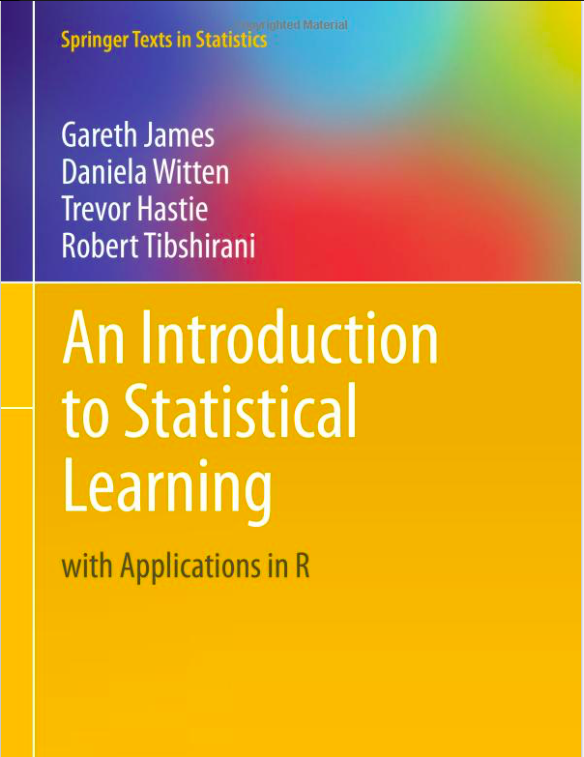
\includegraphics[width=0.1\linewidth]{book1}
        \end{tabular} & 
        \begin{tabular}{l}
            \parbox{0.75\linewidth}{
            \emph{An Introduction to Statistical Learning}\\ Friedman, Hastie, and Tibshirani
            }
        \end{tabular}
    \end{tabular} \\
    \vspace{1ex}
    \begin{tabular}{cl}  
        \begin{tabular}{c}
            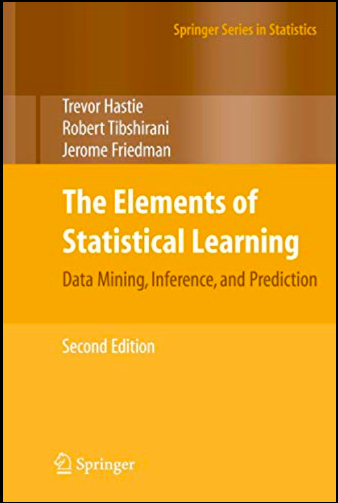
\includegraphics[width=0.1\linewidth]{book2}
        \end{tabular} & 
        \begin{tabular}{l}
            \parbox{0.75\linewidth}{
            \emph{The Elements of Statistical Learning }\\ James, Witten, Hastie, and Tibshirani
            }
        \end{tabular}
    \end{tabular} \\
    \vspace{1ex}
    
\end{frame}

\begin{frame}\frametitle{Software}
    We will use the Python programming language in this course \\
    \vspace{2ex}
    Why Python?
    \begin{itemize}
        \item Python is free and open source
        \item Python is powerful and flexible
        \begin{itemize}
            \item Basic statistics, data cleaning, linear regression, matrix algebra, simulation methods, structural estimation, data visualization, etc.
        \end{itemize}
        \item Well-integrated with app
        \item Easy to deploy algorithm
        \item Python is favored by employers
    \end{itemize}
    \vspace{2ex}
    How can I learn Python?
    \begin{itemize}
        \item Python tutorial in Week 1{\&}2
        \item Many Python resources available for free
        \item First problem set will be a (relatively) gentle introduction to Python
    \end{itemize}
\end{frame}

\begin{frame}\frametitle{Installing Python}
    Installing Python is \emph{usually} straightforward \\
    \vspace{1ex}
    \begin{tabular}{@{\extracolsep{-2ex}} c l}
        \begin{tabular}{c}
            
\includegraphics[width=0.05\linewidth]{jupyter}
        \end{tabular} & 
        \begin{tabular}{l}
            \parbox{0.9\linewidth}{
            \href{https://www.anaconda.com/products/individual/}{Download (\texttt{anaconda.com/products/individual})} and it will include Python and Jupyter Notebook
            }
        \end{tabular}
    \end{tabular} \\
    \vspace{1ex}
    \vspace{3ex}
    What is the difference between Python and Anaconda Jupyter Notebook? \\
    \vspace{1ex}
    \begin{tabular}{@{\extracolsep{-2ex}} c l}
        \begin{tabular}{c}
            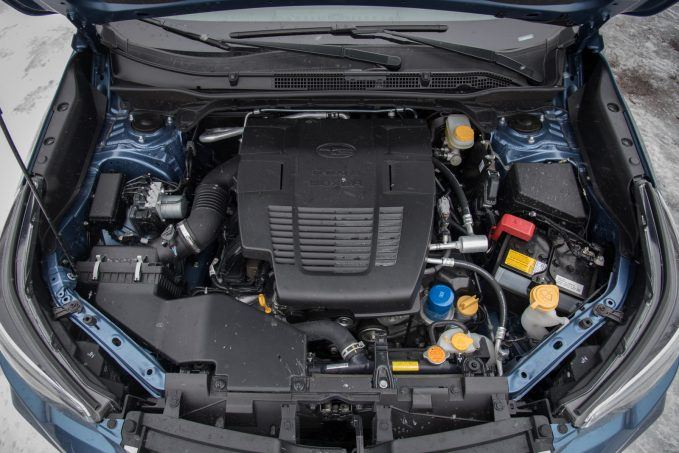
\includegraphics[width=0.25\linewidth]{engine}
        \end{tabular} & 
        \begin{tabular}{l}
            \parbox{0.65\linewidth}{
            Python is like a car's engine. It is the program that powers your data analysis.
            }
        \end{tabular}
    \end{tabular} \\
    \vspace{1ex}
    \begin{tabular}{@{\extracolsep{-2ex}} c l}
        \begin{tabular}{c}
            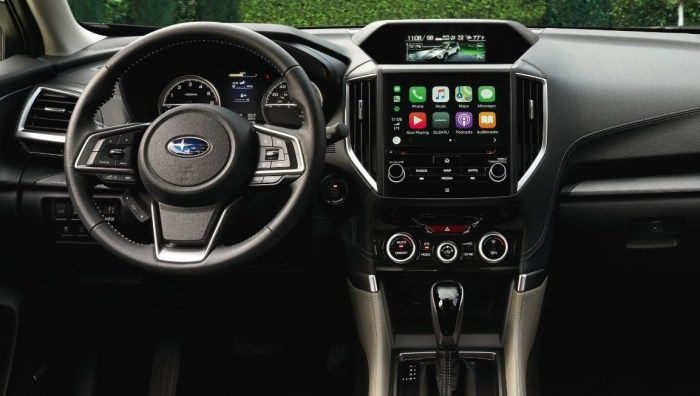
\includegraphics[width=0.25\linewidth]{dashboard}
        \end{tabular} & 
        \begin{tabular}{l}
            \parbox{0.65\linewidth}{
            Jupyter Notebook is like a car's dashboard. It is the program you interact with to harness the power of your ``engine.''
            }
        \end{tabular}
    \end{tabular}
\end{frame}

\section{Grades and Assignments}
\label{grades}
\begin{frame}\frametitle{}
    \vfill
    \centering
    \begin{beamercolorbox}[center]{title}
        \Large Grades and Assignments
    \end{beamercolorbox}
    \vfill
\end{frame}

\begin{frame}\frametitle{Grades}
    The grading policy is as follow:
    \begin{itemize}
        \item Assignments: 30\% (best 6 out of 7)
        \item Midterm: 30\%
        \item Final project: 40\% (Paper 20\%, Presentation 20\%)
    
    \end{itemize}
    
\end{frame}

\begin{frame}\frametitle{Assignments}

 Students are also expected to submit biweekly assignments in which they apply the practiced methods to a pre-defined problem. 
 \begin{itemize}
        \item Apply the ML methods you learn in class
        \item Consist of programming tasks designed to give you experience working with big and otherwise challenging data in the context of econometric analysis
        \item Interpret your results
\end{itemize}
\vspace{2ex}

    Rules for Assignments
    \begin{itemize}
        \item All assignments are due by Monday, 11:59 pm on the week listed in the syllabus
        \item You must submit your code with your write up
        \item Assignments will be evaluated based on both functionality and the readability/organization of the code that you write
    \end{itemize}
    \vspace{2ex}
    See syllabus for tentative problem set schedule
\end{frame}

\begin{frame}\frametitle{Final Project}
    Final project will be similar to problem sets
    \begin{itemize}
        \item Estimation, interpretation, etc.
        \item One month to complete
        \item Work in groups of up to three people
    \end{itemize}
    \vspace{2ex}
    How the final project differs from problem sets
    \begin{itemize}
        \item Closely mimics a real-world research project
        \item Will require roughly twice the effort of a assignment
    \end{itemize}
    \vspace{2ex}
    More details to come toward the end of the semester
\end{frame}

\begin{frame}\frametitle{Participation}
    Participation is required
    \begin{itemize}
        \item Read the assigned reading
        \item Do the assignments
        \item Keep up with in-class discussions and exercises
    \end{itemize}
    \begin{itemize}
        \item  Stay at home if you are sick! Please refer to http://coronavirus.fullerton.edu/mandatory-health-screening/ for recommended steps
        \item  The University requests that any employee or student who tests positive for COVID-19 or becomes aware that they may have been in close contact with someone who either has tested positive for or is suspected to have COVID-19 report the positive result or exposure using the CSUF COVID-19 Self-Reporting Form (http://coronavirus.fullerton.edu/report-covid-19-case-or-exposure/). CSUF’s Infectious Diseases Response Team reviews and verifies COVID-19 confirmed cases and responds to concerns from the campus community on COVID-19.
    \end{itemize}
\end{frame}

\end{document}